\chapter{Computational Homology} \label{ch:homology}

As large amounts of data become available, it becomes more difficult to determine what information is relevant. There are, of course, high and low-level approaches. A high-level approach like a fingerprint scanner or handwriting recognition might be the end-goal of one's analysis, but lower-level approaches like homology look at the geometric makeup of an object and are often a requisite step toward building higher-level processes. Homology is one way of analyzing \textit{local} properties in order to extract information about \textit{global} phenomena.

	At this time, computational homology is a relatively new field and its application in physics has only recently been explored\rf{krishan_2007,gameiro_2004,kurtuldu_2011,mischaikow_2006}. Although homology is a field of algebraic topology, it combines the mathematics of several other fields including combinatorics and computation. The mathematical formalism behind homology is difficult to grasp so only the relevant information will be detailed in \refsect{sect:homologyoverview}. For the interested reader, \refsect{ch2:cubicalhomology} presents a more thorough discussion of the mathematical background of cubical homology.
		
\section{Homology overview} \label{sect:homologyoverview}

At its root, homology is concerned with the enclosed \textit{holes} and connected \textit{pieces} in topological spaces. This vague statement might lead one to ask what exactly we mean by ``connected pieces'' and ``holes''. To gain an intuitive understanding, examine \refFig{fig:reedgriffin} in which the connected pieces (the black segments) and holes (the white enclosed areas) of the Reed Griffin have been colored in. While it may seem easy enough to simply count these structures as I have done, the goal of homology is to provide a formal mathematical description of these geometric structures regardless of the complexity or spatial dimension. Although the formalism of homology is difficult to understand, the relevant concepts are easily illustrated through examples. It's best to think about this in one dimension first.
%
\begin{figure}[h]
	\centering
	\begin{subfigure}[b]{0.3\textwidth}
		
\includegraphics[width=\textwidth]{reedgriffin_notransp.png}
		\caption{} \label{fig:reedgriffin_orig}
	\end{subfigure} \quad
	\begin{subfigure}[b]{0.3\textwidth}
		
\includegraphics[width=\textwidth]{reedgriffin_b0.png}
		\caption{} \label{fig:reedgriffin_b0}
	\end{subfigure} \quad
	\begin{subfigure}[b]{0.3\textwidth}
		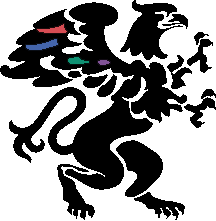
\includegraphics[width=\textwidth]{reedgriffin_b1.png}
		\caption{} \label{fig:reedgriffin_b1}
	\end{subfigure}
	\caption{The homology of the Reed Griffin. On the left (\ref{fig:reedgriffin_orig}) is the original image. The isolated black segments of the Griffin are the ``connected pieces'' and the white enclosed areas are the ``holes''. The other two (\ref{fig:reedgriffin_b0} and \ref{fig:reedgriffin_b1}) have been colored in to highlight the 14 connected pieces and 4 holes respectively. Homology provides a precise mathematical description these structures.} \label{fig:reedgriffin}
\end{figure}
%

\refFig{fig:homology1d} shows two simple topological spaces, $X$ and $Y$. Although $X$ and $Y$ are spaces with one and two line segments respectively, in terms of homology one would say $X$ consists of a single \textit{connected piece} while $Y$ has two distinct pieces. The fact that the line segments are straight or of different length is not important for the homology. In this one-dimensional example, the \textit{zeroth homology groups} of each are
%
\begin{align}
	& H_0(X) \cong \mathbf{Z}^1 \quad \text{and} \quad H_0(Y) \cong \mathbf{Z}^2,
	\label{eq:homology1d}
\end{align}
%
where $\mathbf{Z}$ is the group of integers. The homology pairs a topological space (e.g.\ $X$ and $Y$) with an \textit{abelian group}, a set of elements combined with operations that satisfy five axioms: closure, associativity, identity, invertibility, and commutativity (a full definition can be found in~\refAppe{ap:abeliandef}). Notice, however, that the \textit{zeroth homology group} of $Y$ is $\mathbf{Z}^2$; the rank of the group, $2$, is what accounts for the two distinct pieces, but more on this later.

\begin{figure}[h]
	\begin{center}
		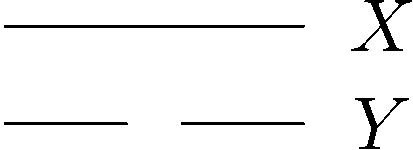
\includegraphics[width=0.3\columnwidth]{Figs/homology1d.pdf}
		\caption{\label{fig:homology1d} Topological spaces $X$ and $Y$. $X$ consists of one connected line segment and $Y$ has two disconnected line segments.}
	\end{center}
\end{figure}

Since there is a \textit{zeroth homology group}, it makes sense that there would be a \textit{first homology group}. Looking at the two-dimensional example in \refFig{fig:homology2d}, the homology of each space $X_a$, $X_b$, $X_c$, and $X_d$ is
%
\begin{align}
	& H_0(X_a) \cong \mathbf{Z} \quad H_0(X_b) \cong \mathbf{Z} \quad H_0(X_c) \cong \mathbf{Z} \quad H_0(X_d) \cong \mathbf{Z^2} \\
	& H_1(X_a) \cong  \mathbf{Z} \quad H_1(X_b) \cong 0 \quad H_1(X_c) \cong \mathbf{Z} \quad H_1(X_d) \cong \mathbf{Z}.
	 \label{eq:homology2d} 
\end{align}

\begin{figure}[h]
	\centering
	\begin{subfigure}[b]{0.2\textwidth}
		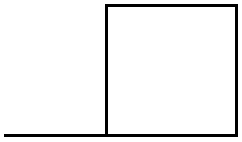
\includegraphics[width=\textwidth]{Figs/homology2d-a.pdf}
		\caption{$X_a$} \label{fig:homology2d-a}
	\end{subfigure} \qquad
	\begin{subfigure}[b]{0.2\textwidth}
		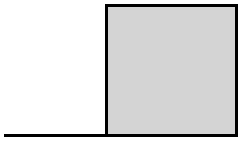
\includegraphics[width=\textwidth]{Figs/homology2d-b.pdf}
		\caption{$X_b$} \label{fig:homology2d-b}
	\end{subfigure} \\
	\begin{subfigure}[b]{0.2\textwidth}
		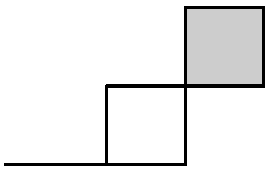
\includegraphics[width=\textwidth]{Figs/homology2d-c.pdf}
		\caption{$X_c$} \label{fig:homology2d-c}
	\end{subfigure} \qquad
	\begin{subfigure}[b]{0.2\textwidth}
		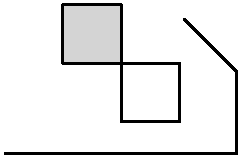
\includegraphics[width=\textwidth]{Figs/homology2d-d.pdf}
		\caption{$X_d$} \label{fig:homology2d-d}
	\end{subfigure}
	\caption{Topological spaces $X_a$, $X_b$, $X_c$, and $X_d$. Shading indicates that the enclosed area is filled.} \label{fig:homology2d}
\end{figure}

Spaces $X_a$, $X_b$, and $X_c$ have a \textit{zeroth homology group} of $\mathbf{Z}$ since there is a single connected component while $X_d$ has $\mathbf{Z^2}$ to account for the two disconnected lines. In each space, a connected component forms an enclosed area (\ie the squares). The square in \refFig{fig:homology2d-a} forms a hole, a region completely enclosed by the black line. Figures~\ref{fig:homology2d-a}, \ref{fig:homology2d-c}, and \ref{fig:homology2d-d} each contain one hole. The shading in Figures~\ref{fig:homology2d-b}, \ref{fig:homology2d-c}, and \ref{fig:homology2d-d} indicates that the hole is filled and is thus no longer counted. Just as the \textit{zeroth homology group} is concerned with connected segments, the \textit{first homology group} is concerned with holes.

The terms ``piece'' and ``hole'' are informal. Formally, we could say that the $k^{th}$ homology group, $H_k(X)$, represents the group of $k$-dimensional holes of $X$ where a $k = 0$ hole is merely the gap between two components (\eg $Y$ in \refFig{fig:homology1d}). As I alluded to earlier, the the rank of the homology group (\eg the rank $2$ of $\mathbf{Z}^2$ in \refeq{eq:homology1d}) represents the \emph{number} of $k$ dimensional holes.\footnote{The ``dimension'' of $k$ is different from the dimension of the topological space. To describe the dimension of a space such as a cube in $\mathbb{R}^3$, call it $X$, we write $\dim X = 3$. Structures of lower dimensions, such as the square faces that make up the cube, are \textit{embedded} in the higher dimensional space $X$. For $k \geq \dim X$, $H_k(X) = 0$ since there are no structures embedded in a space with a higher dimension than that of the space itself. It is important to note that if we could place the topological spaces shown in \refFig{fig:homology2d}, which live in $\mathbb{R}^2$ on the page, into 3-dimensional space, $\mathbb{R}^3$, this would not change the homology groups.} This is called the \textit{Betti number} $\beta_k$. Indeed, Betti numbers are non-zero for all $k < d$ where $d$ is the dimension of the topological space. Betti numbers are the most important feature of the homology in this thesis since they assign a nice mathematical quantity to an otherwise visual characteristic of a topological space. \refFig{fig:kappaV_color} gives the Betti numbers for pattern $\kappa$; there is clearly one single connected component, shown in black, and nine enclosed holes which have been colored in. Thus, $\beta_0 = 1$ and $\beta_1 = 9$.
%
\begin{figure}
	\centering
	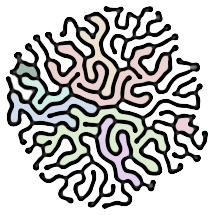
\includegraphics[width=0.3\columnwidth]{kappaV_color.png}
	\caption{\label{fig:kappaV_color} The pattern $\kappa$ described in \refsect{sect:gsmodel}. The homology of $\kappa$ gives Betti numbers $\beta_0 = 1$ and $\beta_1 = 9$. True to the homology, we can easily count a single black connected component and nine holes, each of which is filled with a different color to illustrate this fact.}
\end{figure}

\subsection{Prior work}

Although the literature surrounding homology is relatively little, the techniques described here have been used to characterize complex patterns. Prior work by Gameiro and Mischaikow examines the 1D Gray-Scott system as well as the 2D FitzHugh-Nagumo model\rf{gameiro_2004}. Using a time series of Betti numbers, they are able to calculate the maximal Lyapunov exponent (LE) which, if positive, implies existence of spatial-temporal chaos. They compare their computation of the LE using a time series of Betti numbers to that obtained through standard methods. The results are compelling for two reasons; one is that there is near-perfect agreement between the LE obtained through the Betti time series and standard methods which confirms that using homology data is an acceptable approach. The other is that, due to its topological features, the homology data is also able to capture spatial chaos which the LE calculated through the standard method does not (it only measures temporal chaos).

The work done by Gameiro, Mischaikow, and others provides a wonderful backdrop and inspiration for the analysis of the 2D Gray-Scott model in this thesis. The computational method for calculating homology data of this system is outlined in \refChapter{ch:methods}. In \refsect{sect:entropy}, I describe how this can be used to derive information about the complexity of a system's dynamics.

\section{Cubical homology} \label{ch2:cubicalhomology}

In cubical homology, topological spaces are represented as a collection of cubes. This thesis is concerned with the interpretation of digital images as topological spaces. Digital images are quite literally a collection of two-dimensional cubes, \textit{pixels}, thus a homology that examines these objects is a natural environment for examining the output of computer simulations. In this section, I present a brief mathematical description of cubical homology that closely follows that of\rf{gameiro_2005} and\rf{kaczynski_2007}. By skipping this section, one would miss some of the interesting subtleties of homology theory but a thorough understanding is by no means essential to the understanding of this thesis.

We'll start by defining elementary cubes, which make up the building blocks for the theory. It is important to keep in mind here that one of the fundamental ideas in homology theory is to connect topological objects (\eg connected pieces and holes) to algebraic objects.

\begin{defn}
	An \textit{elementary interval} is an interval $I \subset \R$ of the form
	\begin{align*}
		I = [ l, l+1 ] \quad \text{or} \quad I = [l,l]
	\end{align*}
	for some $l \in \R$. To simplify notation, say $$[l] = [l, l]$$ is an interval containing a single point, which we call a \textit{degenerate} interval. Intervals of the form $[l, l+1]$ are called \textit{nondegenerate}.
\end{defn}

\begin{defn}
	An \textit{elementary cube} $Q$ is a finite cartesian product of elementary intervals, $$ Q = I_1 \times I_2 \times \ldots \times I_d \subset \R^d $$ where each $I_i$ is an elementary interval. We denote the set of all elementary cubes in $\R^d$ as $\Kd$. \\
	The set of all elementary cubes, $\K$, is
	$$ \K := { \bigcup_{d=1}^{\infty} } \Kd . $$
\end{defn}

Two elementary cubes are shown in \refFig{fig:elemcubes}. Cube $Q_1 = [1,2] \times [1,2]$ and $Q_2 = [3,4] \times [1]$. Both $Q_1$ and $Q_2$ are subsets of $\mathbb{R}^2$ even though one interval of $Q_2$ is degenerate.

\begin{figure}
	\centering
	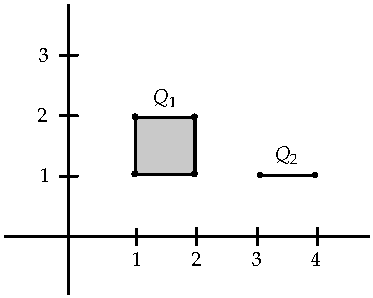
\includegraphics[width=0.4\textwidth]{elemcubes}
	\caption{Two elementary cubes $Q_1, \, Q_2 \subset \mathbb{R}^2.$ The cube $Q_1 = [1,2] \times [1,2]$ and $Q_2 = [3,4] \times [1]$. Notice that $Q_2 \subset \mathbb{R}^2$ is different from the cube $[3,4] \subset \mathbb{R}$ as they are subsets of different spaces.}
	\label{fig:elemcubes}
\end{figure}

\begin{defn}
	Let $Q = I_1 \times I_2 \times \ldots \times I_d \subset \R^d$ be an elementary cube. The \textit{embedding number} of $Q$ is defined to be $d$ which we denote by $\emb{Q}$. Interval $I_i$ is the $i\ith$ \textit{component} of $Q$ and is written $\mathord{I_i(Q)}$. The \textit{dimension} of $Q$ is defined as the number of nondegenerate components in $Q$ and denoted $\dim{Q}$. We refer to an elementary cube $Q$ with $\dim{Q} = k$ as a \textit{k-cube} and denote
	$$ \K_k := \{ Q \in \K | \dim{Q} = k \},$$ and
	$$ \K_{k}^{d} := \K_k \cap \Kd. $$
\end{defn}
The relationship between the embedding number and dimension might be a little muddy since it seems that they would always be the same. Observe that for elementary cube {Q}, if $\emb{Q} = d$, then $Q \in \Kd$. The only general relation between the embedding number and dimension of $Q$ is that $$ 0 \leq \dim{Q} \leq \emb{Q} .$$ To illustrate this, imagine a Rubik's cube on a desk. The Rubik's cube itself has both $\text{emb}, \dim = 3$ while any one square \textit{face} has $\text{emb} = 3$ but $\dim = 2$ (also see \refEx{ex:embvsdim}).

\begin{exmp} \label{ex:embvsdim}
	Given elementary cube $Q := [1,2] \times [1,2] \times [-1] \subset \R^3$, we have $I_1(Q) = [1,2]$, $I_2(Q) = [1,2]$, and $I_3(Q) = [-1]$ (which is degenerate). Therefore, $\emb{Q} = 3$ and $\dim{Q} = 2$, due to the degenerate $I_3$.
\end{exmp}

Now we must define the class of topological spaces for which we define the homology.

\begin{defn}
	A set $X \subset \R^d$ is \textit{cubical complex} if $X$ can be written as a finite union of elementary cubes.
\end{defn}

Given cubical complex $X \subset \R^d$, we define
	$$ \K(X) := \{ Q \in \K \, | \, Q \subset X \} $$ and
	$$ \K_k (X) := \{ Q \in \K (X) \, | \, \dim{Q} = k \}. $$
We can write $\Kd (X)$ to remind us that $X \subset \R^d$ as well as $\Kd_k := \Kd(X) \cap K_k(X)$. For example, elements of $\K_0(X)$ are \textit{vertices} of $X$, elements of $\K_1(X)$ are \textit{edges} and so forth. $\K_k(X)$ are the \textit{k-cubes} of $X$.

Once again, our goal is to establish a relationship between algebraic objects and topological spaces. The first step, then, is to associate some algebraic object with the elementary cubes that we just defined.
%
\begin{defn}
	For each elementary \textit{k-cube} $Q \in \Kd_k$, we associate an algebraic object $\Qhat$ which we call an \textit{elementary k-chain} of $\R^d$ where $\Qhat : \Kd_k \rightarrow \Z$ is the function defined by
	$$\Qhat(P) =
		\begin{cases}
			1	& \text{if } P = Q, \\
			0	& \text{otherwise.}
		\end{cases}$$
	We also define $\wh{0} : \Kd_k \rightarrow \Z$ to be the zero function, \ie~$\wh{0}(Q) = 0$ for all $Q \in \Kd_k$.
	The set of all \textit{elementary k-chains} of $\R^d$ is given by
	$$ \wh{\Kd_k} := \left\{ \Qhat \, | \, Q \in \Kd_k \right\} $$ and the set of all \textit{elementary chains} of $\R^d$ is given by
	$$ \wh{\Kd} := { \bigcup_{k=0}^{\infty} } \wh{\Kd_k} . $$
\end{defn}

As previously mentioned, the purpose of defining the $k$-chain $\wh{Q}$ versus $k$-cube $Q$ is to bridge the gap between the algebra and the topology. Just as a $k$-cube describes a structure formed by the product of intervals (\eg $[0,1] \times [0,1]$ is an elementary 2-cube), a $k$-chain describes a combination of \textit{simplices} (a 0-simplex is a point, a 1-simplex is a segment, a 2-simplex is a triangle, and so on). In the context of a graph, a chain might describe a path between vertices (0-simplices) in the form of a linear combination of the vertices.

For an elementary cube $Q$, we refer to $\Qhat$ as its \textit{dual elementary chain}. Conversely, given elementary chain $\Qhat$, we call $Q$ is its \textit{dual elementary cube}. What we want is a one-to-one relationship between the elementary \textit{k-cubes} (topological objects) and \textit{elementary k-chains} (algebraic objects). In other words, the map of \textit{k-cubes} ($\Kd_k$) to \textit{k-chains} ($\wh{\Kd_k}$) is a \textit{bijection}. 
%
\begin{prop} \label{prop:bijection}
	The map $\phi : \Kd_k \rightarrow \wh{\Kd_k}$ given by $\phi(Q) = \Qhat$ is a bijection.
\end{prop}
%
\begin{proof}
	See Kaczynski \etal\rf{kaczynski_2007}.
\end{proof}

Proposition~\ref{prop:bijection} allows us invoke the inverse of $\phi$ to go from an algebraic object, the elementary chain $\Qhat$, to a topological set, $Q$. The following definition uses the algebra that we have built up to give the elementary \textit{k-chains} algebraic structure.
%
\begin{defn}
	The group $C_k^d$ of \textit{k-dimensional chains} (or \textit{k-chains}) of $\R^d$ is the free abelian group (see \refAppe{ap:freeabeliandef}) generated by the elementary chains of $\Kd_k$. Thus the elements of $C_k^d$ are functions $c : \Kd_k \rightarrow \Z$ such that $c(Q) = 0$ for all but a finite number of elementary cubes $Q \in \Kd_k$. In particular, the set of elementary $k$-chains $\wh{\Kd_k}$ is the basis for $C_k^d$. By the same notation used in \refAppe{ap:abeliandef},
	$$ C_k^d := \Z(\Kd_k). $$
	If $ c \in C_k^d$, then $\dim c := k$.
\end{defn}

\refFig{fig:boundaries} illustrates how we can use information about the boundary to exact information about the $k$-cubes, but we are again using topological information (the existence of a boundary) to derive more topological information (the existence of loops). What we would really like to do is use algebra to get at this information, so we start by defining the algebraic boundary of a $k$-chain.
%
\begin{figure}[h]
	\begin{center}
	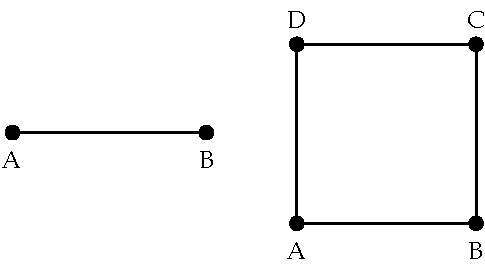
\includegraphics[width=0.5\columnwidth]{boundaries.pdf}
	\caption{\label{fig:boundaries} The line segment (left) has a topological boundary given by $\{ A \} \cup \{ B \}$ (or $[A, B]$) and therefore does not form a loop (a 0-cube). The square (right), however, does not have a boundary (since we can't pick a definite start and end point) and therefore forms a loop (a 1-cube).}
	\end{center}
\end{figure}

The set of elementary chains forms a basis for $C_k^d$, thus we would like to easily describe an arbitrary chain $c \in C_k^d$ in terms of the elements of $\wh{\Kd_k}$. Definition \refeq{defn:chainprod} provides such a relation which is analogous to the dot product in vector space.

\begin{defn} \label{defn:chainprod}
	Consider $c_1, c_2 \in C_k^d$, where $c_1 = \sum_{i=1}^m \alpha_i \Qhat_i $ and $ c_2 = \sum_{i=1}^m \beta_i \Qhat_i $ and $\alpha_i$ and $\beta_i$ scalars. The \textit{scalar product} of the chains $c_1$ and $c_2$ is defined as
	$$ \langle c_1, c_2 \rangle := \sum_{i=1}^m \alpha_i \beta_i . $$
\end{defn}

The astute reader will notice that this definition restricts us to describing a $k$-chain only in terms of $k$-dimensional cubes. We know, however, that cubes may be decomposed into lower dimensional faces. For example, the square in \refFig{fig:boundaries} may be constructed from the four edges (or 1D faces) $[A,B]$, $[B,C]$, $[C,D]$, and $[D,A]$, and we would like to be able to write all $k$-chains in terms of lower-dimensional faces. This will be essential when the boundary operator is defined in \ref{defn:bdop} and provides the motivation for the following definition and proposition.

\begin{defn}
	Given two elementary cubes $P \in \K_{k_1}^{d_1} $ and $ Q \in \K_{k_2}^{d_2} $, let
	$$ \wh{P} \diamond \wh{Q} := \wh{ P \times Q } $$
	This extends to arbitrary chains $ c_1 \in C_{k_1}^{d_1} $ and $ c_2 \in C_{k_2}^{d_2} $ by
	$$ c_1 \diamond c_2 := \sum_{P \in \K_{k_1}, \, Q \in \K_{k_2} } \langle c_1, \wh{P} \rangle \langle c_2, \Qhat \rangle \wh{ P \times Q} $$
	The chain $ c_1 \diamond c_2 \in C_{k_1 + k_2}^{d_1 + d_2} $ is called the \textit{cubical product} of $c_1$ and $c_2$.
\end{defn}

\begin{prop} \label{prop:chainprod}
	Let $\Qhat$ be an elementary cubical chain of $\R^d$ with $d > 1$. Then there exist unique elementary cubical chains $\wh{I}$ and $\wh{P}$ with $\emb{I} = 1$ and $\emb{P} = d - 1$ such that
	$$ \Qhat = \wh{I} \diamond \wh{P} $$
\end{prop}
%
\begin{proof}
	See Kaczynski \etal\rf{kaczynski_2007}.
\end{proof}

\begin{defn} \label{defn:bdop}
	Given $k \in \Z$, the \textit{cubical boundary operator} or \textit{cubical boundary map} given by
	$$ \del_k : C_k^d \rightarrow C_{k-1}^d $$
	is a homomorphism of free abelian groups, which is defined for an elementary chain $\Qhat \in \wh{\Kd_k}$ by induction on the embedding number $d$ as follows. Consider first the case $d = 1$. Then $Q$ is an elementary interval and hence $Q = [l] \in \K_0^1$ or $Q = [l, l+1] \in \K_1^1$ for some $l \in \Z$. Define
		$$ \del_k \Qhat :=
			\begin{cases}
				0	& \text{if } Q = [l], \\
				[ \wh{l+1} ] - [\wh{l}]	& \text{if } Q = [l, l+1]
			\end{cases}$$
	Now assume that $d > 1$. Let $I = I_1(Q)$ and $P = I_2(Q) \times \ldots \times I_d(Q)$. Then by \ref{prop:chainprod},
	$$ \Qhat = \wh{I} \diamond \wh{P}. $$
	Define,
	$$\del_k \Qhat := \del_{k_1} \wh{I} \diamond \wh{P} + (-1)^{k_1} \wh{I} \diamond \del_{k_2} \wh{P}, $$
	where $k_1 = \dim{I}$ and $k_2 = \dim{P}$. Finally, we extend the definition to all chains by linearity; that is, if $c = \alpha_1 \Qhat_1 + \alpha_2 \Qhat_2 + \cdots + \alpha_m \Qhat_m$, then
	$$ \del_k c = \alpha_1 \del_k \Qhat_1 + \alpha_2 \del_k \Qhat_2 + \cdots + \alpha_m \del_k \Qhat_m. $$
\end{defn}

The domain of $\del_k$ is the $k$-chains, so if we know that $c \in C_k^d$, it is redundant and labor intensive to write the subscript $k$ so we simplify to $\del$. Geometrically speaking, the boundary of a $k$-chain is simply the alternating sum of its $(k-1)$-dimensional faces. As \refFig{fig:holes} demonstrates, however, merely having a boundary sum equal to zero is not enough to constitute a loop. The right picture does not characterize a hole since it is filled in by the 2-chain $Q$.\footnote{Not to be confused with 2 Chainz\rf{2chainz}.} This boundary is represented algebraically by $\del (\Qhat) = [\wh{A, B}] + [\wh{B, C}] - [\wh{C, D}] - [\wh{D, A}]$. We would represent the boundary topologically by $[A, B] \cup [B, C] \cup [C, D] \cup [D, A]$.

\begin{figure}[h]
\begin{center}
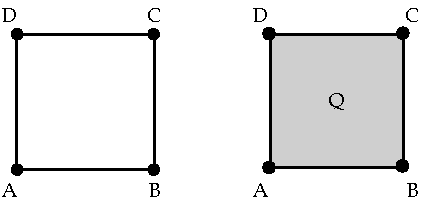
\includegraphics[width=0.5\columnwidth]{holes.pdf}
\caption{\label{fig:holes} The boundary of the chain $[\wh{A, B}] + [\wh{B, C}] - [\wh{C, D}] - [\wh{D, A}]$ is zero in both pictures. The left picture, however, characterizes a loop (or hole) while the one on the right does not since it is ``filled in'' by 2-chain $Q$. }
\end{center}
\end{figure}

We can now say that holes are characterized by chains that have a boundary equal to zero, but are not themselves the boundary of other chains. In order to count the holes, then, we must count the chains which have zero boundary, but are not boundaries. The following definitions help us achieve this.

\begin{defn}
	Let $X \subset \R^d$ be a cubical complex. Let $\wh{\K_k}(X) := \{ \Qhat \, | \, Q \in \K_k(X) \}$. We define the set of $k$-chains of $X$ as the subgroup $C_k(X)$ of $C_k^d$ generated by the elements of $\wh{K_k}(X)$.
\end{defn}

\begin{prop}
	Let $X \subset \R^d$ be a cubical complex. Then
	$$ \del_k (C_k(X)) \subset C_{k-1}(X) $$
\end{prop}

\begin{proof}
	See Kaczynski \etal\rf{kaczynski_2007}.
\end{proof}
%
This leads to the following definition.

\begin{defn}
	The boundary operator of the cubical complex $X$ is defined to be
	$$ \del_k^X : C_k(X) \rightarrow C_{k-1}(X) $$
	obtained by restricting $\del_k : C_k^d \rightarrow C_{k-1}^d$ to $C_k(X)$.
\end{defn}

An extremely important property of the boundary operator is defined in the following proposition.

\begin{prop} \label{prop:bdofbd}
	$$\del \circ \del = 0$$
\end{prop}

\begin{proof}
	See Kaczynski \etal\rf{kaczynski_2007}.
\end{proof}

It should make sense that if we are to take the boundary of a topological object, the boundary itself should have a lower embedding number (the boundary of a square, $k_1=2$, is made up of lines, $k_2=1$). It may not seem immediately intuitive that the boundary of a boundary is zero; the boundary of a disk is a circle which has boundary equal to zero; the boundary of a baseball is its spherical shell which also has a zero boundary. At this point we are tantalizingly close to defining homology---but wait! The following descriptions will be helpful in a moment.

\begin{defn}
	Let $X \subset \R^d$ be a cubical set. A $k$-chain $z \in C_k(X)$ is called a \textit{k-cycle} in $X$ if $\del z = 0$. Thus the set of all $k$-cycles of X is the kernel of $\del_k^X$ and so it is a subgroup of $C_k(X)$. We denote the set of all $k$-cycles by $Z_k(X)$. In short,
	\begin{align}
		Z_k(X) := \text{ker } \del_k^X = C_k(X) \cap \text{ker } \del_k \subset C_k(X).
	\end{align}
\end{defn}

%
A $k$-chain $z \in C_k(X)$ is called a \textit{boundary} in $X$ if there exists a $(k+1)$-chain $c \in C_{k+1}(X)$ such that $\del c = z$. Thus the set of all boundary elements in $C_k(X)$ is the image\footnote{That's ``image'' in the mathematical sense (\ie the subset that contains the output of a function). The shorthand for this is $\text{im} f$ for function $f$.} of $\del_{k+1}^X$, and so it is also a subgroup of $C_k(X)$. We denote the set of all boundary elements in $C_k(X)$ by $B_k(X)$. Once again,
%
\begin{align}
	B_k(X) := \text{im } \del_{k+1}^X = \del_{k+1} (C_{k+1}(X)) \subset C_k(X).
\end{align}
%
We can now say more precisely what we wanted before; we want to characterize holes by chains that have zero boundary (\ie $k$-cycles, the elements of $Z_k(X)$) but are not themselves the boundary of other chains. The set of all $k$-chains that represent boundaries of other chains is $B_k(X)$, so we want to count the elements of $Z_k(X)$ that are not in $B_k(X)$, and this will define our set of $k$-dimensional holes. This  is easily done by taking the quotient group of $Z_k(X)$ by $B_k(X)$ but this requires that $B_k(X)$ be a subgroup of $Z_k(X)$. By Proposition~\ref{prop:bdofbd}, $\del c = z$ implies $\del z = \del^2 c = 0$, therefore every boundary is a cycle and $B_k(X)$ is a subgroup of $Z_k(X)$ so we may rightfully proceed to the most important definition of this section.

\begin{defn}
	The $k\ith$ \textit{cubical homology group} of $X$ is the quotient group
	$$ H_k(X) := Z_k(X) / B_k(X). $$
	The homology of $X$ is the collection of all homology groups of $X$. The shorthand for this is
	$$ H_{*}(X) := \{ H_k(X) \}_{k \in \Z} .$$
\end{defn}%

For a cubical set $X \subset \R^d$ we can show that, for $i = 0, \ldots, d-1$, 
$$H_i(X) = \Z^{\beta_i} \oplus \Z_{b_1} \oplus \Z_{b_2} \oplus \cdots \oplus \Z_{b_k},$$ 
where $\beta_i$ is a nonnegative integer, $\Z_b$ is the group of integers modulo $b$, $b_i > 1$ provided $k > 0$, and $b_i$ divides $b_{i+1}$ for $i \in \{ 1, 2, \ldots, k-1 \}$ provided $k > 1$. The $\oplus$ operator denotes a direct sum. For $ i \geq d$ we have $H_i(X) = 0$.

Integer $\beta_i$ is known as the $i\ith$ \textit{Betti number} of $X$ and $b_1, b_2, \ldots, b_k$ are the \textit{torsion coefficients} of $H_i(X)$. In general, $\beta_i := \text{rank}( H_i( X ) )$. Spaces with dimension $d \leq 3$ do not have torsion coefficients, just $H_i(X) = \Z^{\beta_i}$, so we need not worry about them for our purposes\rf{gameiro_2005}.

This is certainly a great abstraction from what we started with before, connected pieces and holes in a topological space, but here is some geometrical intuition. As previously indicated, the Betti numbers encode some geometrical information. $\beta_0$ is equal to the number of connected pieces of $X$, $\beta_1$ is the number of holes (or loops) if $d = 2$ or the number of tunnels if $d = 3$. $\beta_2$ equals the number of cavities if $d=3$.

\begin{exmp}
	An ordinary bike tube (a torus) has $\beta_0 = 1$, the single connected piece of rubber; $\beta_1 = 1$, one hole in the center; and $\beta_2 = 1$, the hollow cavity inside the tube.
\end{exmp}

The mathematical tour-de-force that we've just undertaken might seem like major overkill. After all, here we are merely concerned with counting geometric structures that could theoretically be eyeballed (tedious as that may be). I argue, however, that the homology maintains some nice features for us. For one, it provides a mathematically rigorous definition of the structures in question. Furthermore, the homology of any structure is unchanged in any higher-dimensional space (\eg~the homology groups of an empty square are the same in $\mathbb{R}^2$ as in $\mathbb{R}^3$ or $\mathbb{R}^4$ for that matter). Homology is not concerned with size or shape of any object either; the homology of a coffee mug is identical to that of \refFig{fig:homology2d-a}. The theory reduces the amount of information required to describe an object to a few topological quantities which may be difficult to grasp visually. Analysis of higher dimensional data, such as a 4D construction of medical imaging data, which would require a great amount of thought to assess visually, is completely feasible through cubical homology\rf{kaczynski_2007}. Due to its dimension-independent formulation, the applications of cubical homology are limited only by the ability to construct sensical topological information. In the following chapter, we shall see how the homology theory described here can be applied to analyze patterns of the Gray-Scott system.


